\documentclass[tikz,border=12pt]{standalone}
\usepackage[T1]{fontenc}
\usepackage{mathptmx}
\usepackage{tikz}
\usetikzlibrary{arrows.meta,positioning,shapes.misc,calc}

\definecolor{boxfill}{HTML}{EEECFE}
\definecolor{boxdraw}{HTML}{5B4B8A}
\definecolor{altfill}{HTML}{F8F7FD}
\definecolor{altdraw}{HTML}{7A6EB0}

\begin{document}
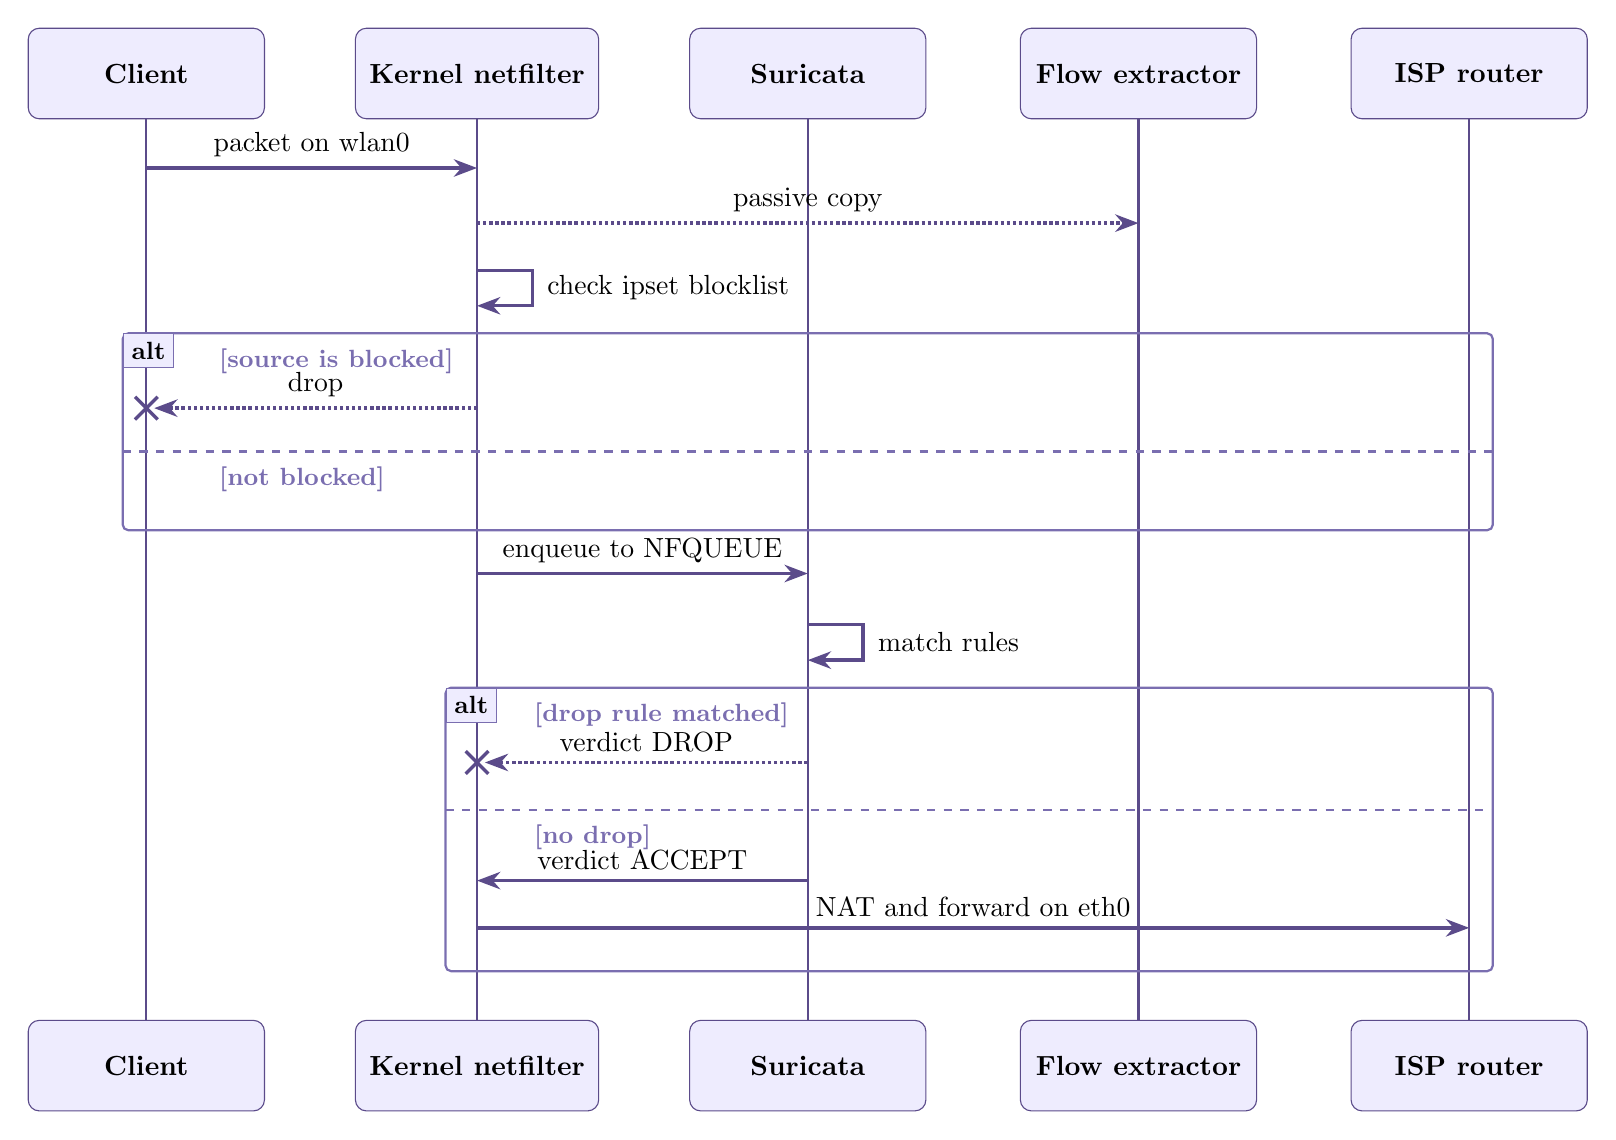
\begin{tikzpicture}[
  font=\normalsize,
  >=Stealth,
  actor/.style={draw=boxdraw, fill=boxfill, rounded corners=4pt,
    align=center, minimum width=3.0cm, minimum height=1.15cm, font=\normalsize\bfseries, inner sep=5pt},
  lifeline/.style={draw=boxdraw, thick},
  msg/.style={->, very thick, draw=boxdraw},
  dmsg/.style={->, very thick, densely dotted, draw=boxdraw},
  looparr/.style={->, very thick, draw=boxdraw},
  cross/.style={cross out, draw=boxdraw, very thick, minimum size=7pt, inner sep=0pt}
]

\def\topY{0}
\def\botY{-12.6}

% Lifelines and Actor headers
\foreach \name/\x/\label in {
  c/0/Client,
  k/4.2/Kernel netfilter,
  s/8.4/Suricata,
  f/12.6/Flow extractor,
  i/16.8/ISP router} {
  \node[actor] (\name) at (\x,\topY) {\label};
  \node[actor] (\name b) at (\x,\botY) {\label};
  \draw[lifeline] (\name.south) -- (\name b.north);
}

% 1. packet on wlan0
\draw[msg] (0,-1.2) -- node[above, font=\normalsize] {packet on wlan0} (4.2,-1.2);

% 2. passive copy
\draw[dmsg] (4.2,-1.9) -- node[above, font=\normalsize] {passive copy} (12.6,-1.9);

% 3. check ipset blocklist (self-loop)
\draw[looparr] (4.2,-2.5) -- ++(0.7,0) -- ++(0,-0.45) -- ++(-0.7,0);
\node[right=2pt, font=\normalsize, anchor=west] at (4.9,-2.72) {check ipset blocklist};

% 4. alt block 1: source blocked vs not blocked
\draw[draw=altdraw, thick, rounded corners=2pt] (-0.3,-3.3) rectangle (17.1,-5.8);
\node[draw=altdraw, fill=boxfill, inner sep=3pt, font=\small\bfseries, anchor=north west]
  at (-0.3,-3.3) {alt};

% [source is blocked]
\node[font=\small\bfseries, text=altdraw, anchor=west] at (0.8,-3.65) {[source is blocked]};
\draw[dmsg] (4.2,-4.25) -- node[above, font=\normalsize] {drop} (0.1,-4.25);
\node[cross] at (0,-4.25) {};

% dashed divider
\draw[altdraw, dashed, thick] (-0.3,-4.8) -- (17.1,-4.8);

% [not blocked]
\node[font=\small\bfseries, text=altdraw, anchor=west] at (0.8,-5.15) {[not blocked]};

% 5. enqueue to NFQUEUE
\draw[msg] (4.2,-6.35) -- node[above, font=\normalsize] {enqueue to NFQUEUE} (8.4,-6.35);

% 6. match rules (self-loop)
\draw[looparr] (8.4,-7.0) -- ++(0.7,0) -- ++(0,-0.45) -- ++(-0.7,0);
\node[right=2pt, font=\normalsize, anchor=west] at (9.1,-7.22) {match rules};

% 7. alt block 2: drop rule matched vs no drop
\draw[draw=altdraw, thick, rounded corners=2pt] (3.8,-7.8) rectangle (17.1,-11.4);
\node[draw=altdraw, fill=boxfill, inner sep=3pt, font=\small\bfseries, anchor=north west]
  at (3.8,-7.8) {alt};

% [drop rule matched]
\node[font=\small\bfseries, text=altdraw, anchor=west] at (4.8,-8.15) {[drop rule matched]};
\draw[dmsg] (8.4,-8.75) -- node[above, font=\normalsize] {verdict DROP} (4.3,-8.75);
\node[cross] at (4.2,-8.75) {};

% dashed divider
\draw[altdraw, dashed, thick] (3.8,-9.35) -- (17.1,-9.35);

% [no drop]
\node[font=\small\bfseries, text=altdraw, anchor=west] at (4.8,-9.7) {[no drop]};
\draw[msg] (8.4,-10.25) -- node[above, font=\normalsize] {verdict ACCEPT} (4.2,-10.25);
\draw[msg] (4.2,-10.85) -- node[above, font=\normalsize] {NAT and forward on eth0} (16.8,-10.85);

\end{tikzpicture}
\end{document}
